\documentclass{standalone}
\usepackage{tikz}
\usetikzlibrary{patterns, positioning}
\usepackage[sfdefault]{ClearSans} %% option 'sfdefault' activates Clear Sans as the default text font
\usepackage[T1]{fontenc}

\begin{document}
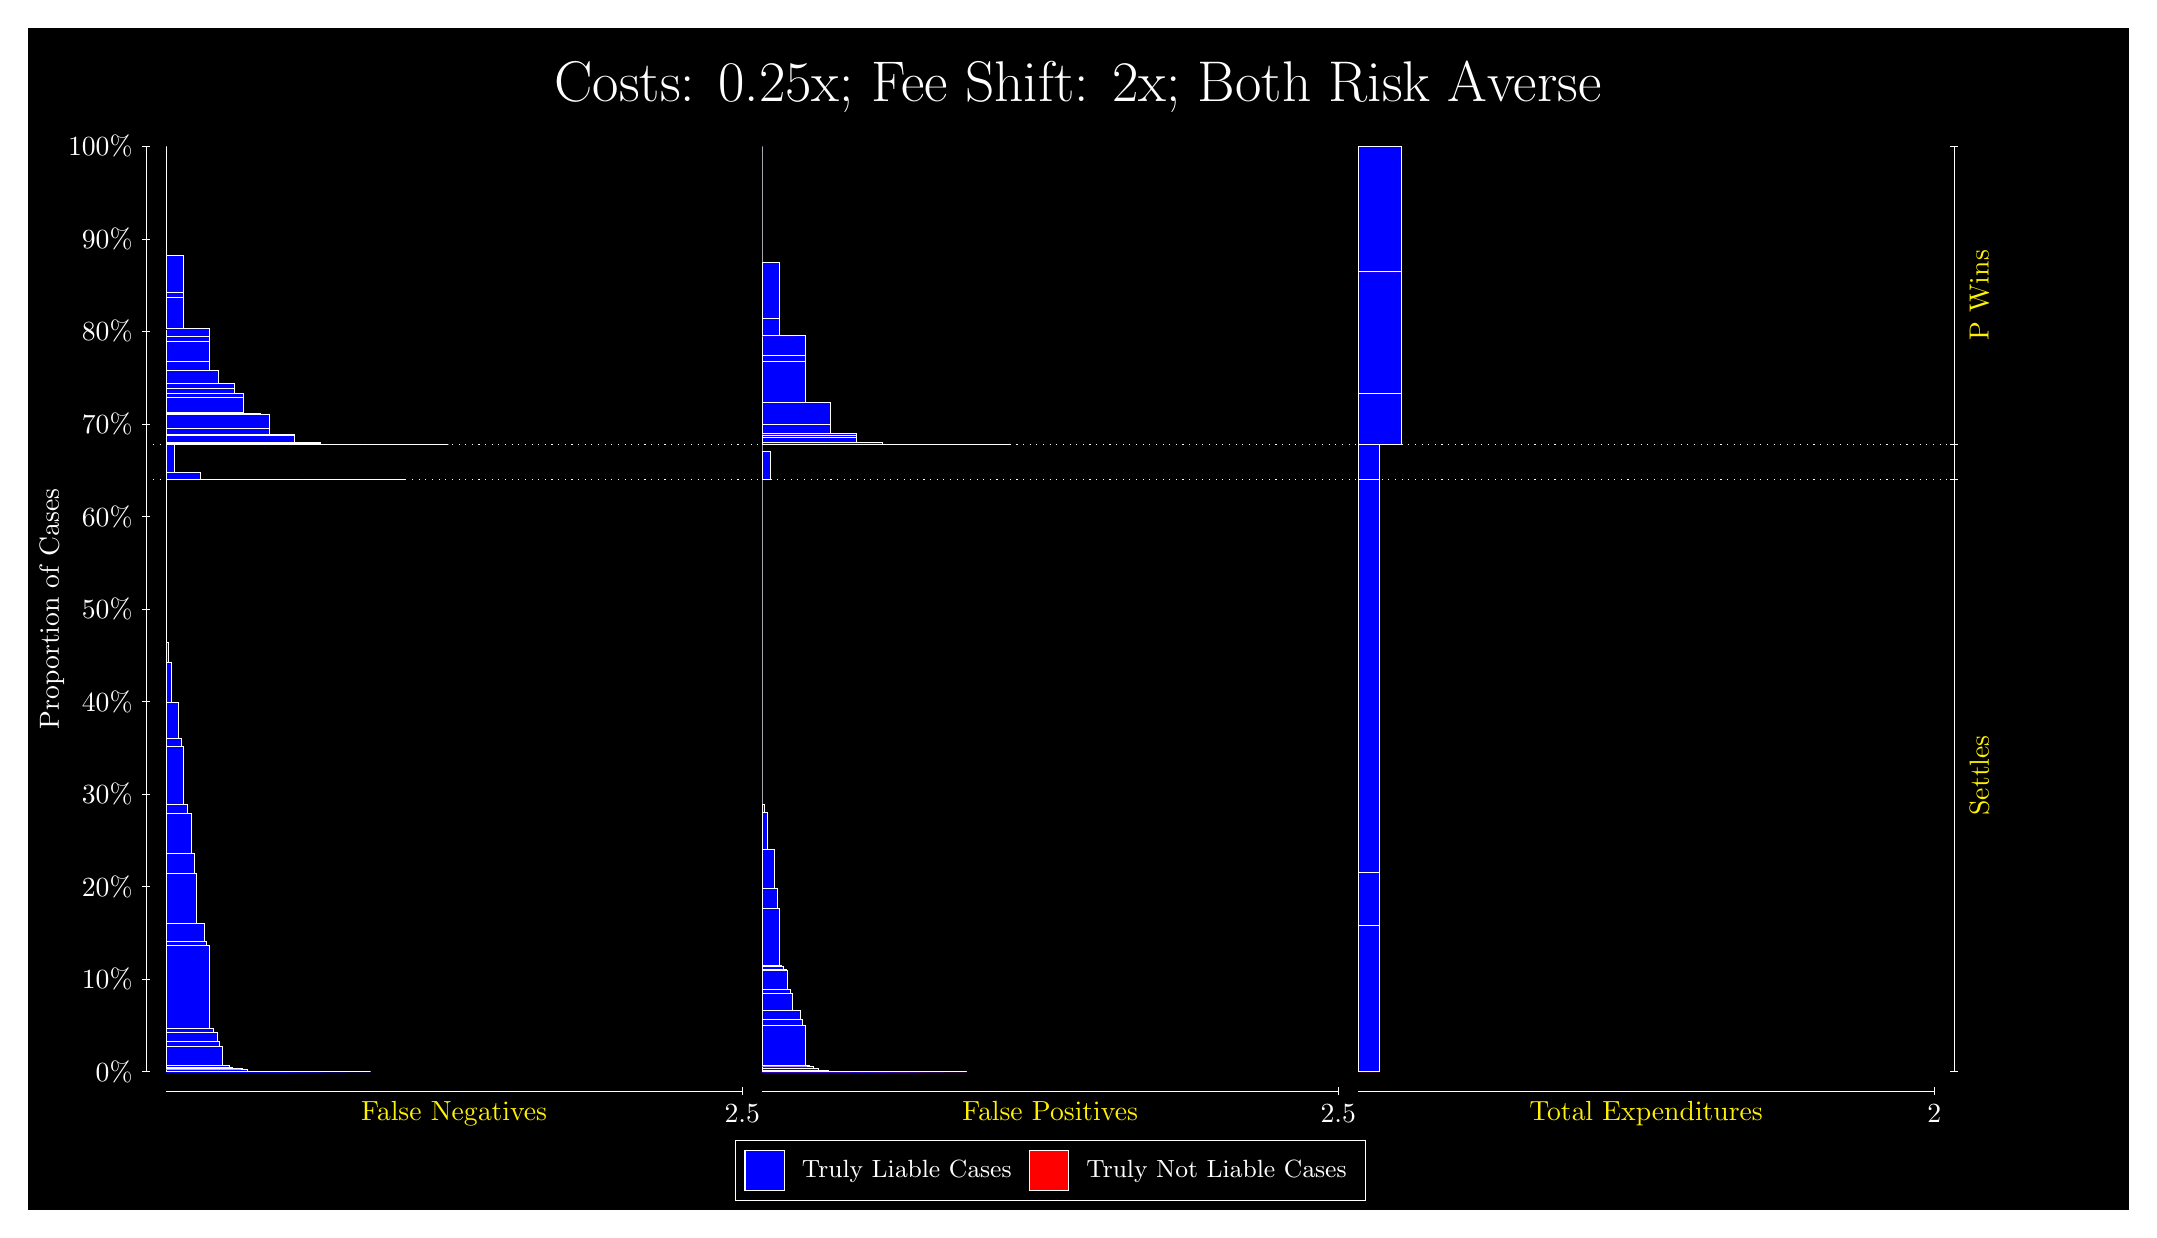
\begin{tikzpicture}
\draw[fill=black] (0,0) rectangle (26.667,15);
\draw[text=white] (0,13.5) rectangle (26.667,15) node[midway] {\huge Costs: 0.25x; Fee Shift: 2x; Both Risk Averse};
\draw[white, very thin] (1.5,1.75) -- (1.5,13.5);
\node[rotate=90, text=white, anchor=center] at (0.3, 7.625) {Proportion of Cases};
\draw[white, very thin] (1.45,1.75) -- (1.55,1.75);
\node[text=white, anchor=east] at (1.45, 1.75) {0\%};
\draw[white, very thin] (1.45,2.925) -- (1.55,2.925);
\node[text=white, anchor=east] at (1.45, 2.925) {10\%};
\draw[white, very thin] (1.45,4.1) -- (1.55,4.1);
\node[text=white, anchor=east] at (1.45, 4.1) {20\%};
\draw[white, very thin] (1.45,5.275) -- (1.55,5.275);
\node[text=white, anchor=east] at (1.45, 5.275) {30\%};
\draw[white, very thin] (1.45,6.45) -- (1.55,6.45);
\node[text=white, anchor=east] at (1.45, 6.45) {40\%};
\draw[white, very thin] (1.45,7.625) -- (1.55,7.625);
\node[text=white, anchor=east] at (1.45, 7.625) {50\%};
\draw[white, very thin] (1.45,8.8) -- (1.55,8.8);
\node[text=white, anchor=east] at (1.45, 8.8) {60\%};
\draw[white, very thin] (1.45,9.975) -- (1.55,9.975);
\node[text=white, anchor=east] at (1.45, 9.975) {70\%};
\draw[white, very thin] (1.45,11.15) -- (1.55,11.15);
\node[text=white, anchor=east] at (1.45, 11.15) {80\%};
\draw[white, very thin] (1.45,12.325) -- (1.55,12.325);
\node[text=white, anchor=east] at (1.45, 12.325) {90\%};
\draw[white, very thin] (1.45,13.5) -- (1.55,13.5);
\node[text=white, anchor=east] at (1.45, 13.5) {100\%};

\draw[white, very thin] (24.457,1.75) -- (24.457,13.5);
\draw[white, very thin] (24.407,1.75) -- (24.507,1.75);
\node[anchor=west] at (24.407, 1.75) {};
\draw[white, very thin] (24.407,9.2723) -- (24.507,9.2723);
\node[anchor=west] at (24.407, 9.2723) {};
\draw[white, very thin] (24.407,9.7159) -- (24.507,9.7159);
\node[anchor=west] at (24.407, 9.7159) {};
\draw[white, very thin] (24.407,13.5) -- (24.507,13.5);
\node[anchor=west] at (24.407, 13.5) {};

\draw[white, very thin, fill=blue] (1.75,1.75) rectangle (4.3482,1.75);
\draw[white, very thin, fill=blue] (1.75,1.75) rectangle (4.0554,1.75);
\draw[white, very thin, fill=blue] (1.75,1.75) rectangle (4.0229,1.75);
\draw[white, very thin, fill=blue] (1.75,1.75) rectangle (3.7627,1.75);
\draw[white, very thin, fill=blue] (1.75,1.75) rectangle (3.7302,1.75);
\draw[white, very thin, fill=blue] (1.75,1.75) rectangle (3.6976,1.75);
\draw[white, very thin, fill=blue] (1.75,1.75) rectangle (3.6163,1.75);
\draw[white, very thin, fill=blue] (1.75,1.75) rectangle (3.4374,1.75);
\draw[white, very thin, fill=blue] (1.75,1.75) rectangle (3.4049,1.75);
\draw[white, very thin, fill=blue] (1.75,1.75) rectangle (3.3723,1.75);
\draw[white, very thin, fill=blue] (1.75,1.75) rectangle (3.3236,1.75);
\draw[white, very thin, fill=blue] (1.75,1.75) rectangle (3.291,1.75);
\draw[white, very thin, fill=blue] (1.75,1.75) rectangle (3.1121,1.7505);
\draw[white, very thin, fill=blue] (1.75,1.7505) rectangle (3.0796,1.7506);
\draw[white, very thin, fill=blue] (1.75,1.7506) rectangle (3.0471,1.7506);
\draw[white, very thin, fill=blue] (1.75,1.7506) rectangle (3.0308,1.7506);
\draw[white, very thin, fill=blue] (1.75,1.7506) rectangle (2.9983,1.7507);
\draw[white, very thin, fill=blue] (1.75,1.7507) rectangle (2.9657,1.7507);
\draw[white, very thin, fill=blue] (1.75,1.7507) rectangle (2.8844,1.7517);
\draw[white, very thin, fill=blue] (1.75,1.7517) rectangle (2.7868,1.7759);
\draw[white, very thin, fill=blue] (1.75,1.7759) rectangle (2.7543,1.7809);
\draw[white, very thin, fill=blue] (1.75,1.7809) rectangle (2.7218,1.7861);
\draw[white, very thin, fill=blue] (1.75,1.7861) rectangle (2.7055,1.7863);
\draw[white, very thin, fill=blue] (1.75,1.7863) rectangle (2.673,1.7909);
\draw[white, very thin, fill=blue] (1.75,1.7909) rectangle (2.6405,1.7911);
\draw[white, very thin, fill=blue] (1.75,1.7911) rectangle (2.5917,1.8006);
\draw[white, very thin, fill=blue] (1.75,1.8006) rectangle (2.5591,1.8278);
\draw[white, very thin, fill=blue] (1.75,1.8278) rectangle (2.4616,2.0712);
\draw[white, very thin, fill=blue] (1.75,2.0712) rectangle (2.429,2.1392);
\draw[white, very thin, fill=blue] (1.75,2.1392) rectangle (2.3965,2.2488);
\draw[white, very thin, fill=blue] (1.75,2.2488) rectangle (2.3802,2.251);
\draw[white, very thin, fill=blue] (1.75,2.251) rectangle (2.3477,2.2999);
\draw[white, very thin, fill=blue] (1.75,2.2999) rectangle (2.3152,2.3021);
\draw[white, very thin, fill=blue] (1.75,2.3021) rectangle (2.2989,3.3541);
\draw[white, very thin, fill=blue] (1.75,3.3541) rectangle (2.2664,3.4102);
\draw[white, very thin, fill=blue] (1.75,3.4102) rectangle (2.2339,3.6349);
\draw[white, very thin, fill=blue] (1.75,3.6349) rectangle (2.1363,4.2708);
\draw[white, very thin, fill=blue] (1.75,4.2708) rectangle (2.1037,4.5191);
\draw[white, very thin, fill=blue] (1.75,4.5191) rectangle (2.0712,5.0284);
\draw[white, very thin, fill=blue] (1.75,5.0284) rectangle (2.055,5.0336);
\draw[white, very thin, fill=blue] (1.75,5.0336) rectangle (2.0224,5.141);
\draw[white, very thin, fill=blue] (1.75,5.141) rectangle (1.9899,5.1463);
\draw[white, very thin, fill=blue] (1.75,5.1463) rectangle (1.9736,5.8765);
\draw[white, very thin, fill=blue] (1.75,5.8765) rectangle (1.9411,5.9852);
\draw[white, very thin, fill=blue] (1.75,5.9852) rectangle (1.9086,6.4439);
\draw[white, very thin, fill=blue] (1.75,6.4439) rectangle (1.811,6.9471);
\draw[white, very thin, fill=blue] (1.75,6.9471) rectangle (1.7785,7.1985);
\draw[white, very thin, fill=red] (1.75,7.1985) rectangle (1.75,7.1985);
\draw[white, very thin, fill=blue] (1.75,7.1985) rectangle (1.75,9.2723);
\draw[white, very thin, fill=blue] (1.75,9.2723) rectangle (4.7873,9.2723);
\draw[white, very thin, fill=blue] (1.75,9.2723) rectangle (4.462,9.2723);
\draw[white, very thin, fill=blue] (1.75,9.2723) rectangle (4.1368,9.2723);
\draw[white, very thin, fill=blue] (1.75,9.2723) rectangle (3.8115,9.2723);
\draw[white, very thin, fill=blue] (1.75,9.2723) rectangle (3.4862,9.2723);
\draw[white, very thin, fill=blue] (1.75,9.2723) rectangle (3.1609,9.2723);
\draw[white, very thin, fill=blue] (1.75,9.2723) rectangle (2.8356,9.2724);
\draw[white, very thin, fill=blue] (1.75,9.2724) rectangle (2.5103,9.2768);
\draw[white, very thin, fill=blue] (1.75,9.2768) rectangle (2.1851,9.3556);
\draw[white, very thin, fill=blue] (1.75,9.3556) rectangle (1.8598,9.7159);
\draw[white, very thin, fill=red] (1.75,9.7159) rectangle (1.75,9.7159);
\draw[white, very thin, fill=blue] (1.75,9.7159) rectangle (5.3362,9.7159);
\draw[white, very thin, fill=blue] (1.75,9.7159) rectangle (5.011,9.7159);
\draw[white, very thin, fill=blue] (1.75,9.7159) rectangle (4.6857,9.716);
\draw[white, very thin, fill=blue] (1.75,9.716) rectangle (4.5718,9.716);
\draw[white, very thin, fill=blue] (1.75,9.716) rectangle (4.3604,9.7162);
\draw[white, very thin, fill=blue] (1.75,9.7162) rectangle (4.2465,9.7162);
\draw[white, very thin, fill=blue] (1.75,9.7162) rectangle (4.2465,9.7162);
\draw[white, very thin, fill=blue] (1.75,9.7162) rectangle (4.0351,9.7179);
\draw[white, very thin, fill=blue] (1.75,9.7179) rectangle (4.0351,9.7191);
\draw[white, very thin, fill=blue] (1.75,9.7191) rectangle (3.9213,9.7191);
\draw[white, very thin, fill=blue] (1.75,9.7191) rectangle (3.7098,9.7293);
\draw[white, very thin, fill=blue] (1.75,9.7293) rectangle (3.7098,9.7425);
\draw[white, very thin, fill=blue] (1.75,9.7425) rectangle (3.596,9.7425);
\draw[white, very thin, fill=blue] (1.75,9.7425) rectangle (3.3845,9.833);
\draw[white, very thin, fill=blue] (1.75,9.833) rectangle (3.3845,9.849);
\draw[white, very thin, fill=blue] (1.75,9.849) rectangle (3.2707,9.849);
\draw[white, very thin, fill=blue] (1.75,9.849) rectangle (3.2707,9.849);
\draw[white, very thin, fill=blue] (1.75,9.849) rectangle (3.0593,9.9135);
\draw[white, very thin, fill=blue] (1.75,9.9135) rectangle (3.0593,10.101);
\draw[white, very thin, fill=blue] (1.75,10.101) rectangle (2.9454,10.105);
\draw[white, very thin, fill=blue] (1.75,10.105) rectangle (2.9454,10.112);
\draw[white, very thin, fill=blue] (1.75,10.112) rectangle (2.9454,10.112);
\draw[white, very thin, fill=blue] (1.75,10.112) rectangle (2.734,10.117);
\draw[white, very thin, fill=blue] (1.75,10.117) rectangle (2.734,10.317);
\draw[white, very thin, fill=blue] (1.75,10.317) rectangle (2.734,10.365);
\draw[white, very thin, fill=blue] (1.75,10.365) rectangle (2.6201,10.366);
\draw[white, very thin, fill=blue] (1.75,10.366) rectangle (2.6201,10.422);
\draw[white, very thin, fill=blue] (1.75,10.422) rectangle (2.6201,10.489);
\draw[white, very thin, fill=blue] (1.75,10.489) rectangle (2.4087,10.65);
\draw[white, very thin, fill=blue] (1.75,10.65) rectangle (2.2948,10.769);
\draw[white, very thin, fill=blue] (1.75,10.769) rectangle (2.2948,11.021);
\draw[white, very thin, fill=blue] (1.75,11.021) rectangle (2.2948,11.093);
\draw[white, very thin, fill=blue] (1.75,11.093) rectangle (2.2948,11.183);
\draw[white, very thin, fill=blue] (1.75,11.183) rectangle (2.0834,11.185);
\draw[white, very thin, fill=blue] (1.75,11.185) rectangle (2.0834,11.185);
\draw[white, very thin, fill=blue] (1.75,11.185) rectangle (1.9696,11.582);
\draw[white, very thin, fill=blue] (1.75,11.582) rectangle (1.9696,11.652);
\draw[white, very thin, fill=blue] (1.75,11.652) rectangle (1.9696,12.121);
\draw[white, very thin, fill=blue] (1.75,12.121) rectangle (1.7581,12.121);
\draw[white, very thin, fill=blue] (1.75,12.121) rectangle (1.7581,12.121);
\draw[white, very thin, fill=red] (1.75,12.121) rectangle (1.75,12.121);
\draw[white, very thin, fill=blue] (1.75,12.121) rectangle (1.75,13.5);
\draw[white, very thin, fill=red] (9.3189,1.75) rectangle (11.917,1.75);
\draw[white, very thin, fill=blue] (9.3189,1.75) rectangle (11.917,1.75);
\draw[white, very thin, fill=red] (9.3189,1.75) rectangle (11.624,1.75);
\draw[white, very thin, fill=blue] (9.3189,1.75) rectangle (11.624,1.75);
\draw[white, very thin, fill=blue] (9.3189,1.75) rectangle (11.592,1.75);
\draw[white, very thin, fill=red] (9.3189,1.75) rectangle (11.332,1.75);
\draw[white, very thin, fill=blue] (9.3189,1.75) rectangle (11.332,1.75);
\draw[white, very thin, fill=blue] (9.3189,1.75) rectangle (11.299,1.75);
\draw[white, very thin, fill=blue] (9.3189,1.75) rectangle (11.266,1.75);
\draw[white, very thin, fill=red] (9.3189,1.75) rectangle (11.185,1.75);
\draw[white, very thin, fill=blue] (9.3189,1.75) rectangle (11.185,1.75);
\draw[white, very thin, fill=blue] (9.3189,1.75) rectangle (11.006,1.75);
\draw[white, very thin, fill=blue] (9.3189,1.75) rectangle (10.974,1.75);
\draw[white, very thin, fill=blue] (9.3189,1.75) rectangle (10.941,1.75);
\draw[white, very thin, fill=red] (9.3189,1.75) rectangle (10.892,1.75);
\draw[white, very thin, fill=blue] (9.3189,1.75) rectangle (10.892,1.75);
\draw[white, very thin, fill=blue] (9.3189,1.75) rectangle (10.86,1.75);
\draw[white, very thin, fill=blue] (9.3189,1.75) rectangle (10.681,1.75);
\draw[white, very thin, fill=blue] (9.3189,1.75) rectangle (10.648,1.75);
\draw[white, very thin, fill=blue] (9.3189,1.75) rectangle (10.616,1.75);
\draw[white, very thin, fill=red] (9.3189,1.75) rectangle (10.6,1.75);
\draw[white, very thin, fill=blue] (9.3189,1.75) rectangle (10.6,1.75);
\draw[white, very thin, fill=blue] (9.3189,1.75) rectangle (10.567,1.75);
\draw[white, very thin, fill=blue] (9.3189,1.75) rectangle (10.535,1.75);
\draw[white, very thin, fill=red] (9.3189,1.75) rectangle (10.453,1.75);
\draw[white, very thin, fill=blue] (9.3189,1.75) rectangle (10.453,1.7501);
\draw[white, very thin, fill=blue] (9.3189,1.7501) rectangle (10.356,1.7506);
\draw[white, very thin, fill=blue] (9.3189,1.7506) rectangle (10.323,1.7507);
\draw[white, very thin, fill=blue] (9.3189,1.7507) rectangle (10.291,1.7512);
\draw[white, very thin, fill=blue] (9.3189,1.7512) rectangle (10.274,1.7512);
\draw[white, very thin, fill=blue] (9.3189,1.7512) rectangle (10.242,1.7512);
\draw[white, very thin, fill=blue] (9.3189,1.7512) rectangle (10.209,1.7512);
\draw[white, very thin, fill=red] (9.3189,1.7512) rectangle (10.161,1.7512);
\draw[white, very thin, fill=blue] (9.3189,1.7512) rectangle (10.161,1.7617);
\draw[white, very thin, fill=blue] (9.3189,1.7617) rectangle (10.128,1.7677);
\draw[white, very thin, fill=blue] (9.3189,1.7677) rectangle (10.03,1.7914);
\draw[white, very thin, fill=blue] (9.3189,1.7914) rectangle (9.9979,1.7959);
\draw[white, very thin, fill=blue] (9.3189,1.7959) rectangle (9.9654,1.82);
\draw[white, very thin, fill=blue] (9.3189,1.82) rectangle (9.9491,1.8202);
\draw[white, very thin, fill=blue] (9.3189,1.8202) rectangle (9.9166,1.8248);
\draw[white, very thin, fill=blue] (9.3189,1.8248) rectangle (9.884,1.825);
\draw[white, very thin, fill=red] (9.3189,1.825) rectangle (9.8678,1.825);
\draw[white, very thin, fill=blue] (9.3189,1.825) rectangle (9.8678,2.3341);
\draw[white, very thin, fill=blue] (9.3189,2.3341) rectangle (9.8353,2.4122);
\draw[white, very thin, fill=blue] (9.3189,2.4122) rectangle (9.8027,2.5231);
\draw[white, very thin, fill=blue] (9.3189,2.5231) rectangle (9.7051,2.745);
\draw[white, very thin, fill=blue] (9.3189,2.745) rectangle (9.6726,2.7939);
\draw[white, very thin, fill=blue] (9.3189,2.7939) rectangle (9.6401,3.0403);
\draw[white, very thin, fill=blue] (9.3189,3.0403) rectangle (9.6238,3.0426);
\draw[white, very thin, fill=blue] (9.3189,3.0426) rectangle (9.5913,3.0915);
\draw[white, very thin, fill=blue] (9.3189,3.0915) rectangle (9.5588,3.0937);
\draw[white, very thin, fill=blue] (9.3189,3.0937) rectangle (9.5425,3.8239);
\draw[white, very thin, fill=blue] (9.3189,3.8239) rectangle (9.51,4.0752);
\draw[white, very thin, fill=blue] (9.3189,4.0752) rectangle (9.4774,4.5784);
\draw[white, very thin, fill=blue] (9.3189,4.5784) rectangle (9.3799,5.0371);
\draw[white, very thin, fill=blue] (9.3189,5.0371) rectangle (9.3473,5.1459);
\draw[white, very thin, fill=blue] (9.3189,5.1459) rectangle (9.3189,9.2723);
\draw[white, very thin, fill=red] (9.3189,9.2723) rectangle (9.4287,9.2723);
\draw[white, very thin, fill=blue] (9.3189,9.2723) rectangle (9.4287,9.6327);
\draw[white, very thin, fill=blue] (9.3189,9.6327) rectangle (9.3189,9.7159);
\draw[white, very thin, fill=red] (9.3189,9.7159) rectangle (12.466,9.7159);
\draw[white, very thin, fill=blue] (9.3189,9.7159) rectangle (12.466,9.7159);
\draw[white, very thin, fill=red] (9.3189,9.7159) rectangle (12.141,9.7159);
\draw[white, very thin, fill=blue] (9.3189,9.7159) rectangle (12.141,9.7159);
\draw[white, very thin, fill=red] (9.3189,9.7159) rectangle (11.815,9.7159);
\draw[white, very thin, fill=blue] (9.3189,9.7159) rectangle (11.815,9.7159);
\draw[white, very thin, fill=blue] (9.3189,9.7159) rectangle (11.815,9.716);
\draw[white, very thin, fill=blue] (9.3189,9.716) rectangle (11.49,9.716);
\draw[white, very thin, fill=red] (9.3189,9.716) rectangle (11.49,9.716);
\draw[white, very thin, fill=blue] (9.3189,9.716) rectangle (11.49,9.7161);
\draw[white, very thin, fill=red] (9.3189,9.7161) rectangle (11.165,9.7161);
\draw[white, very thin, fill=blue] (9.3189,9.7161) rectangle (11.165,9.7183);
\draw[white, very thin, fill=red] (9.3189,9.7183) rectangle (10.84,9.7183);
\draw[white, very thin, fill=blue] (9.3189,9.7183) rectangle (10.84,9.7387);
\draw[white, very thin, fill=red] (9.3189,9.7387) rectangle (10.726,9.7387);
\draw[white, very thin, fill=blue] (9.3189,9.7387) rectangle (10.726,9.7387);
\draw[white, very thin, fill=red] (9.3189,9.7387) rectangle (10.514,9.7387);
\draw[white, very thin, fill=blue] (9.3189,9.7387) rectangle (10.514,9.8048);
\draw[white, very thin, fill=blue] (9.3189,9.8048) rectangle (10.514,9.8293);
\draw[white, very thin, fill=blue] (9.3189,9.8293) rectangle (10.514,9.8516);
\draw[white, very thin, fill=blue] (9.3189,9.8516) rectangle (10.4,9.8516);
\draw[white, very thin, fill=red] (9.3189,9.8516) rectangle (10.4,9.8516);
\draw[white, very thin, fill=blue] (9.3189,9.8516) rectangle (10.4,9.8516);
\draw[white, very thin, fill=red] (9.3189,9.8516) rectangle (10.189,9.8516);
\draw[white, very thin, fill=blue] (9.3189,9.8516) rectangle (10.189,9.9749);
\draw[white, very thin, fill=blue] (9.3189,9.9749) rectangle (10.189,10.25);
\draw[white, very thin, fill=blue] (9.3189,10.25) rectangle (10.075,10.25);
\draw[white, very thin, fill=red] (9.3189,10.25) rectangle (10.075,10.25);
\draw[white, very thin, fill=blue] (9.3189,10.25) rectangle (10.075,10.25);
\draw[white, very thin, fill=red] (9.3189,10.25) rectangle (9.8637,10.25);
\draw[white, very thin, fill=blue] (9.3189,10.25) rectangle (9.8637,10.776);
\draw[white, very thin, fill=blue] (9.3189,10.776) rectangle (9.8637,10.841);
\draw[white, very thin, fill=blue] (9.3189,10.841) rectangle (9.8637,11.095);
\draw[white, very thin, fill=blue] (9.3189,11.095) rectangle (9.7499,11.095);
\draw[white, very thin, fill=red] (9.3189,11.095) rectangle (9.7499,11.095);
\draw[white, very thin, fill=blue] (9.3189,11.095) rectangle (9.7499,11.095);
\draw[white, very thin, fill=blue] (9.3189,11.095) rectangle (9.5384,11.313);
\draw[white, very thin, fill=blue] (9.3189,11.313) rectangle (9.5384,12.031);
\draw[white, very thin, fill=blue] (9.3189,12.031) rectangle (9.4246,12.031);
\draw[white, very thin, fill=red] (9.3189,12.031) rectangle (9.4246,12.031);
\draw[white, very thin, fill=blue] (9.3189,12.031) rectangle (9.4246,12.032);
\draw[white, very thin, fill=blue] (9.3189,12.032) rectangle (9.4246,12.033);
\draw[white, very thin, fill=red] (9.3189,12.033) rectangle (9.3189,12.033);
\draw[white, very thin, fill=blue] (9.3189,12.033) rectangle (9.3189,13.5);
\draw[white, very thin, fill=red] (16.888,1.75) rectangle (17.162,1.75);
\draw[white, very thin, fill=blue] (16.888,1.75) rectangle (17.162,3.6135);
\draw[white, very thin, fill=red] (16.888,3.6135) rectangle (17.162,3.6135);
\draw[white, very thin, fill=blue] (16.888,3.6135) rectangle (17.162,4.2748);
\draw[white, very thin, fill=red] (16.888,4.2748) rectangle (17.162,4.2748);
\draw[white, very thin, fill=blue] (16.888,4.2748) rectangle (17.162,9.2723);
\draw[white, very thin, fill=red] (16.888,9.2723) rectangle (17.162,9.2723);
\draw[white, very thin, fill=blue] (16.888,9.2723) rectangle (17.162,9.7159);
\draw[white, very thin, fill=red] (16.888,9.7159) rectangle (17.437,9.7159);
\draw[white, very thin, fill=blue] (16.888,9.7159) rectangle (17.437,10.368);
\draw[white, very thin, fill=red] (16.888,10.368) rectangle (17.437,10.368);
\draw[white, very thin, fill=blue] (16.888,10.368) rectangle (17.437,11.908);
\draw[white, very thin, fill=red] (16.888,11.908) rectangle (17.437,11.908);
\draw[white, very thin, fill=blue] (16.888,11.908) rectangle (17.437,13.5);
\draw[white, dotted] (1.5,9.2723) -- (24.457,9.2723);
\draw[white, dotted] (1.5,9.7159) -- (24.457,9.7159);
\draw[white, very thin] (1.75,1.5) -- (9.0689,1.5);
\node[text=yellow, anchor=north] at (5.4094, 1.5) {False Negatives};
\draw[white, very thin] (9.0689,1.45) -- (9.0689,1.55);
\node[text=white, anchor=north] at (9.0689, 1.45) {2.5};

\draw[white, very thin] (9.3189,1.5) -- (16.638,1.5);
\node[text=yellow, anchor=north] at (12.978, 1.5) {False Positives};
\draw[white, very thin] (16.638,1.45) -- (16.638,1.55);
\node[text=white, anchor=north] at (16.638, 1.45) {2.5};

\draw[white, very thin] (16.888,1.5) -- (24.207,1.5);
\node[text=yellow, anchor=north] at (20.547, 1.5) {Total Expenditures};
\draw[white, very thin] (24.207,1.45) -- (24.207,1.55);
\node[text=white, anchor=north] at (24.207, 1.45) {2};

\node[text=yellow, centered, rotate=90] at (24.777, 5.5112) {Settles};

\node[text=yellow, centered, rotate=90] at (24.777, 11.608) {P Wins};

\draw (12.978300999999998,1.5) node[draw=none] (baseCoordinate) {};
\begin{scope}[align=center]
        \matrix[scale=0.5, draw=white, below=0.5cm of baseCoordinate, nodes={draw}, column sep=0.1cm]{
            \node[rectangle, draw, minimum width=0.5cm, minimum height=0.5cm, fill=blue] {}; &
            \node[draw=none, font=\small, text=white] (B) {Truly Liable Cases}; &
            \node[rectangle, draw, minimum width=0.5cm, minimum height=0.5cm, fill=red] {}; &
            \node[draw=none, font=\small, text=white] (B) {Truly Not Liable Cases}; \\
            };
\end{scope}

\end{tikzpicture}
\end{document}